\section{Grundlagen}\label{Kapitel Grundlagen}
	In diesem Kapitel werden die Grundlagen zur Analyse von Primzahlen und dem diskreten Logarithmus gegeben. Dazu werden im allg. nur die Definitionen und Sätze geliefert. Für Beweise der hier angeführten Sätze sei auf die Bücher \cite{Kryptografie:in:Theorie:und:Praxis}, \cite{Erste:Hilfe:in:Linearer:Algebra}, \cite{Kryptographie:und:IT-Sicherheit} und \cite{Information:und:Kommunikation}
	%\textbf{[TODO noch weiter wenn nötig [x],[y],[z]]}
	verwiesen. Es wird vorausgesetzt, dass die Rechenvorschriften des Modulo bekannt sind.
	
	Für diese Ausarbeitung wurden diverse Quellen unterstützend verwendet. Da es Notationsunterschiede der einzelnen Quellen gibt, führt dies dazu, dass sich nicht an die Notation aller genutzten Quellen gehalten werden kann. Speziell in \cite{Erste:Hilfe:in:Linearer:Algebra} wird eine multiplikative Gruppe aller Einheiten in $G$ mit $G^X$ bezeichnet. Von dieser Notation wird abgesehen und die aus den anderen Quellen weiter verbreitete Notation $G^*$ verwendet.
	
	\subsection{Algebraische Strukturen}
		%TODO wenn nötig und möglich noch mal zu den anderen Struktruen je 1 -2 konkrete Beispiele mit aufnehmen wie bei Halbgruppen
		In diesem Kapitel werden die algebraischen Strukturen: Halbgruppen, Gruppen, Ringe und Körper vorgestellt. Diese werden für ein späteres Kapitel benötigt. Die algebraischen Strukturen beschreiben ein abstraktes Rechnen mit Zahlen. Dies ermöglicht gezielter, nur die Rechenregeln an sich zu untersuchen, unabhängig von der Rechengröße und der jeweiligen Operation. Ein Anwendungsbereich ist u. a. in der Kryptographie zu finden.~\cite{Kryptographie:und:Algorithmen}
	
		\subsubsection{Halbgruppen}
			Eine Halbgruppe ist eine Menge M mit einer assoziativen Operation \mycircOhne, geschrieben mit (M, \mycircOhne) oder einfach nur M. Zur Erinnerung, das Assoziativgesetz besagt: (a \mycirc b) \mycirc c = a \mycirc (b \mycirc c) für alle a, b, c \myin M. Dies gilt für sämtliche Elemente einer Halbgruppe. Das Zeichen \mycirc ist Platzhalter für eine beliebige Operation. Der Wertebereich von \mycirc ist eine Teilmenge von M, sodass a \mycirc b \myin M für alle a, b \myin M gilt. Für das Zeichen \mycirc werden auch die folgenden Operationszeichen verwendet: $*$, \mycdotOhne, +. Auch muss die Menge nicht zwangsläufig M sein.~\cite{Erste:Hilfe:in:Linearer:Algebra}
			
			Durch das Assoziativgesetz können also Klammern weggelassen werden. Zum besseren Verständnis folgen einige konkrete Beispiele von Halbgruppen~\cite{Erste:Hilfe:in:Linearer:Algebra}:
			
			\begin{itemize}
				\item \myMenge{N}, \myMenge{Z}, \myMenge{Q}, \myMenge{R}, \myMenge{C} sind Halbgruppen mit der Addition als Operation, ebenso wie mit der Multiplikation.
				\item Wenn a \mycirc b = |b - a| für alle a, b \myin \myMenge{Z}, dann ist (\myMenge{Z}, \mycircOhne) keine Halbgruppe, da in diesem Fall (1 \mycirc 2) \mycirc 3 = 1 \mycirc 3 = 2 ist, aber 1 \mycirc (2 \mycirc 3) = 1 \mycirc 1 = 0 ist. Ein Verändern der Klammerung ergibt unterschiedliche Ergebnisse. Somit ist das Assoziativgesetz nicht mehr gewährleistet, wodurch \myMenge{Z} in diesem Fall keine Halbgruppe mehr sein kann.
			\end{itemize}

			Sobald es ein neutrales Element in einer Halbgruppe gibt, heißt dieses \textbf{Monoid}. Ein neutrales Element ist immer dann gegeben, wenn es ein e \myin M gibt, sodass für alle a \myin M gilt: a \mycirc e = e \mycirc a = a. Dieses weitere Axiom muss von jeder Halbgruppe erfüllt werden, um ein Monoid zu sein. Als Zeichen für ein Monoid wird neben e oft auch 1 verwendet, bei den Operationszeichen \mycircOhne, \mycdotOhne, $*$. Wird das + als Operationszeichen verwendet, ist oft 0 das neutrale Element.~\cite{Erste:Hilfe:in:Linearer:Algebra}

			Wenn ein Monoid auch das folgende Axiom erfüllt, ist es eine \textbf{Gruppe}. Existiert für alle a \myin G ein b \myin G, sodass a \mycirc b = b \mycirc a = e gilt, so heißt b invers zu a.~\cite{Erste:Hilfe:in:Linearer:Algebra}
		
		\subsubsection{Ringe}
			In einem Ring als algebraische Struktur sind mehr als nur eine Operation vorhanden. Eine Menge R mit den zwei Operationen + und \mycdot auf R ist genau dann ein Ring, wenn die folgenden drei Bedingungen gelten~\cite{Erste:Hilfe:in:Linearer:Algebra}:
			
			\begin{itemize}
				\item (R, +) ist eine abelsche Gruppe. (Eine Operation \mycirc auf einer Menge M heiß kommutativ oder abelsch, wenn a \mycirc b = b \mycirc a für alle a, b \myin M gilt.)
				\item (R, \mycdotOhne) ist ein Monoid
				\item Für alle a, b, c \myin R gilt: a(b + c) = ab + ac, (a + b)c = ac + bc (Distributivgesetze)
			\end{itemize}
			
			Zusätzlich heißt ein Ring kommutativ, wenn die Operation \mycdot kommutativ ist. Ein Ring besitzt also immer eine kommutative Addition und eine nicht notwendigerweise kommutative Multiplikation. Die beiden Distributivgesetze verbinden diese beiden Operationen miteinander. Ein Ring heißt nullteilerfrei wenn a \mycdot b = 0 ist und dadurch impliziert wird, dass a = 0 oder b = 0 sein muss, für alle a, b \myin R. Wenn es für ein a \myin R ein b gibt, so dass ab = ba = 1 gilt, dann ist a invertierbar oder eine Einheit. Alle Elemente im Monoid (R, \mycdotOhne) wo dies zutrifft, sind in einer multiplikativen Gruppe zusammengefasst, und werden als R$^*$ bezeichnet.~\cite{Erste:Hilfe:in:Linearer:Algebra}
			
			Es gibt spezielle Ringe, die sogenannten Körper. Ist eine Menge (K, +, \mycdotOhne) ein Ring und ist ($K / \{0\}$, \mycdotOhne) eine kommutative Gruppe, ist K ein Körper. Alle von Null verschiedenen Elemente sind Einheiten und es gilt: K* = $K / \{0\}$.~\cite{Erste:Hilfe:in:Linearer:Algebra}
			
		\subsubsection{Integritätsbereiche}
			Wie in~\cite{Algorithmische:Zahlentheorie} angegeben ist ein Integritätsbereich ein kommutativer, nullteilerfreier Ring R mit Einselement. Aus dieser Definition ergeben sich die Integritätsbereiche der ganzen Zahlen \myMenge{Z}, der ganzen Gauß’schen Zahlen \myMenge{Z}[i] und des Polynomrings in einem unbestimmten X über einem Körper K, der K[X] bezeichnet wird. 
			\begin{displaymath}
				\mathbb{Z}[i] = \{n + im  \in \mathbb{C} : n,m \in \mathbb{Z}\}
			\end{displaymath}
			\begin{displaymath}	
				K[X] = \{p(X)= a_0 + a_1X + a_2X^2 + . . . + a_nX^n~|~a_i \in K, n \in \mathbb{N}\}					
			\end{displaymath}

			Des weiteren wird ein Integritätsbereich mit einer Funktion  $\beta : R \longrightarrow$ \myMenge{N}, für die gilt: 
			\begin{displaymath}
				\mathrm{x = qy + r,~~~q, r \in R,	mit~r=0~oder~\beta(r) < \beta(y)}
			\end{displaymath}
			als euklidischer Ring bezeichnet und lässt die Division mit Rest zu. Wie in \cite{Algorithmische:Zahlentheorie} gezeigt, ist jeder der Ringe Z, Z[i] und K[X], für einen beliebigen Körper K, euklidisch. Die Erkenntnis, dass es weitere Integritätsbereiche als \myMenge{Z} gibt, wird in den effizienten Primzahltests wieder aufgegriffen. 
			
			Die Teilbarkeit einer Zahl a \myin R durch b \myin R ohne Rest wird b \myTeiler a geschrieben. Kann a durch b nicht ohne Rest geteilt werden, wird b \myNichtTeiler a geschrieben.
		
		\subsubsection{Restklassenringe in \myMenge{Z}}
			Restklassenringe \myMenge{Z}/m\myMenge{Z} oder auch \myMathRM{\mathbb{Z}_m} ergeben sich aus der Definition einer Addition und Multiplikation auf Restklassen. Eine Restklasse bezeichnet zwei Zahlen x, y \myin \myMenge{Z}, die bei der Division durch m \myin \myMenge{N} den gleichen Rest haben. Diese zwei Zahlen sind also in der gleichen Restklasse. Die Anzahl der Restklassen in einem Restklassenring ist gleich m. Die Äquivalenzrelation der beiden Zahlen bezüglich der Restklasse kann wie folgt definiert werden:
			Zwei Zahlen x, y \myin \myMenge{Z} heißen kongruent modulo m \myin \myMenge{N} wenn m \myTeiler $x-y$. In Zeichen:
			\begin{displaymath}
				x \equiv y~mod~m
			\end{displaymath}	
			Die zugehörigen Beweise und Rechenvorschriften für Restklassenringe finden sich in \cite{Algorithmische:Zahlentheorie}.
			
		\subsection{Euklidischer Algorithmus}
			Der euklidische Algorithmus wird zur Berechnung des größten gemeinsamen Teilers zweier Zahlen benötigt. Der Algorithmus findet in fast allen weiteren Betrachtungen Anwendung und wird deshalb explizit angegeben. Wie in \cite{Diskrete:Strukturen} bewiesen, kann der Algorithmus wie folgt definiert werden:
			
			Sind m, n \myin \myMenge{N}\ zwei natürliche Zahlen mit m \myKleinerGleich n und m \myNichtTeiler n, so gilt:
			\begin{displaymath}
				ggT(m, n) = ggT(n~mod~m, m).
			\end{displaymath}
						
		\subsection{Euler’sche \myPhi -Funktion}
			Die Eulersche phi-Funktion \myPhi(m) berechnet die Anzahl teilerfremder Zahlen für eine gegebene Zahl m \myGroesser 1. Also gilt nach \cite{Algorithmische:Zahlentheorie}: 
			\begin{displaymath}
				\varphi(m) = Card((\mathbb{Z}/m\mathbb{Z})^*).
			\end{displaymath}			
			Mit Card(M) ist die Kardinalität der Menge M gemeint. Die Bezeichnung \myMathRM{(\mathbb{Z}/m\mathbb{Z})^*} steht für die Menge der Zahlen aus \myMathRM{\mathbb{Z}/m\mathbb{Z}}, die ein multiplikatives Inverses besitzen. Geschrieben sieht die Menge wie folgt aus:
			\begin{displaymath}
				(\mathbb{Z}/m\mathbb{Z})^* = \mathbb{Z}_m^* = \{a \in \mathbb{Z}_m ~|~ggT(a,m) = 1\}.
			\end{displaymath}
			Die Menge \myMathRM{\mathbb{Z}_m^*} kann auch Einheitengruppe genannt werden. Ein Beispiel für den Restklassenring modulo 10 (\myMathRM{\mathbb{Z}_{10}^*}) sind die Elemente 1, 3, 7 und 9. In \cite{Mathematik:fuer:Informatiker} kann gut nachvollzogen werden, warum ein multiplikatives Inverses von a existiert, wenn der ggT(a,m) = 1 ist.
		
	\subsection{Elliptische Kurven Grundlagen}\label{Elliptischen Kurven Grundlagen}
		In diesem Kapitel sollen nur die Grundlagen von elliptischen Kurven näher gebracht werden, um so die \textbf{E}lliptic \textbf{C}urve \textbf{C}ryptography, kurz \textbf{ECC}, verstehen zu können. Der Vorteil beim ECC-Verfahren im Vergleich zum RSA-Verfahren liegt darin, dass die Schlüssellänge deutlich kürzer ausfallen kann, ohne dabei an Sicherheit zu verlieren. Ein RSA-Schlüssel mit 1024 Bit ist etwa so sicher wie ein Schlüssel aus einer elliptischen Kurve mit gerade mal ca. 160 Bit. Dazu kommt, dass der Rechenaufwand und Speicherbedarf beim ECC-Verfahren wesentlich geringer ist, als beim RSA-Verfahren. So kann ECC in Smartcards und Mobiltelefonen genutzt werden.\cite{Information:und:Kommunikation}
		
		Um die Funktionsweise der elliptischen Kurven in ihrer vollen Breite und Tiefe zu verstehen, ist eine sehr komplexe Mathematik notwendig. Innerhalb dieser Seminararbeit kann dieses Thema nicht breiter und tiefer durchleuchtet werden. Es wird nur ein Teilbereich der elliptischen Kurven betrachtet, der aus kryptografischer Sicht sehr interessant ist. Für weitergehende Informationen sei auf die folgende Literatur verwiesen: \cite{Information:und:Kommunikation} und \cite{Kryptographie:und:IT-Sicherheit}.
		
		Eine elliptische Kurve ist eine ebene Kurve wie in Abbildung~\ref{ABBILDUNG_elliptischenKurveAddition} gezeigt. Sie wird durch eine Gleichung der Form: $y^2 = x^3 + ax +b$ beschrieben. Damit ist eine Menge Z aller Punkte P(x, y), die auf der elliptischen Kurve liegen, definiert. Wichtig dabei ist, dass die Kurvenparameter a und b so gewählt sind, dass die partiellen Ableitungen nach x und nach y auf keinem Punkt der Kurve gleichzeitig null sind. Dazu später mehr.
		
		Das Addieren von zwei Punkten, die auf der elliptischen Kurve liegen, ergibt wieder einen Punkt, welcher ebenfalls auf der Kurve liegt \cite{Information:und:Kommunikation}. Mit Addition ist das Verknüpfen von zwei Punkten gemeint. Man könnte es auch als Multiplikation bezeichnen. In beiden Fällen hat es nichts mit den bekannten Operationen auf Zahlen zu tun. Das Addieren von zwei Punkten ist vielmehr geometrisch definiert, siehe dazu auch Abbildung~\ref{ABBILDUNG_elliptischenKurveAddition}:
		
		\begin{figure}
			\centering
			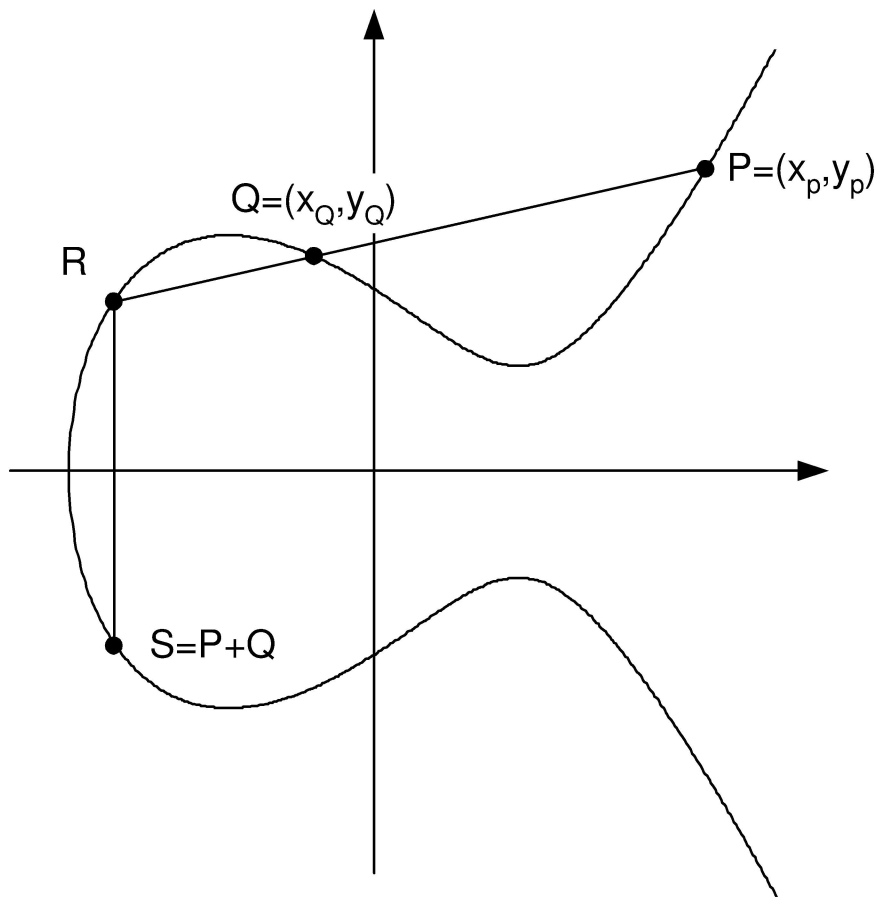
\epsfig{file=includes/images/ElliptischeKurveAddition.PNG, height=3in, width=3in}
			\caption{Addition von zwei Punkten auf einer elliptischen Kurve~\cite{Information:und:Kommunikation}}
			\label{ABBILDUNG_elliptischenKurveAddition}
		\end{figure}
		
		\begin{quote}
			\begin{defi}
				Durch die gegebenen Punkte P und Q wird eine Gerade gelegt, welche die Kurve in einem dritten Punkt R schneidet. Dieser wird anschließend an der x-Achse 
				gespiegelt. Als Ergebnis erhält man den Punkt S, welcher als Addition von P und Q bezeichnet wird.\cite{Information:und:Kommunikation}
			\end{defi}
		\end{quote}
		
		Die so definierte Addition ist kommutativ. Zur Erinnerung: P + Q = Q + P. Nicht für alle elliptischen Kurven kann eine Addition von Punkten durchgeführt werden. Wie oben bereits erwähnt, dürfen die partiellen Ableitungen nach x und nach y auf keinem Punkt der Kurve gleichzeitig null sein. Anders ausgedrückt: Die Kurve darf sich nicht selbst schneiden, ansonsten kann die Additionsoperation nicht für beliebige Punkte durchgeführt werden.
		Zusätzlich muss beachtet werden, dass bei einer Addition von zwei Punkten die nachfolgenden Spezialfälle auftreten können\cite{Information:und:Kommunikation}:
		
		\begin{itemize}
			\item Wenn für die beiden zu addierenden Punkte Q = P gilt, wird die Tangente an der Kurve im Punkt P verwendet. Dabei entsteht der Schnittpunkt mit der Kurve in R und durch Spiegelung resultiert daraus S = P + P = 2P.
			\item Sollten die X-Koordinaten beider zu addierender Punkte gleich sein, sodass (Q\myTiefstellen{X} = P\myTiefstellen{X}) gilt, entsteht eine vertikale Gerade und die Kurve wird kein weiteres Mal geschnitten. Für diesen Fall wird die elliptische Kurve um einen weiteren Punkt \myInftyOhne, welcher im Unendlichen liegt, ergänzt. Die Addition von Punk P mit \myInfty ist so definiert, dass man wiederum P als Ergebnis erhält (P + \myInfty = P). Somit ist \myInfty das neutrale Element der Addition. Es gilt also: P + Q = \myInfty wenn die x-Koordinaten von P und Q gleich sind. Daraus folgt, dass Q das inverse Element von P ist und es gilt: Q = -P.
		\end{itemize}
		
		Das Addieren eines Punktes P mit einem Skalar k \myin \{1, 2, 3 ...\} wird als wiederholte Addition definiert:
		
		\begin{displaymath}
			kP = P1 + P2 + ... + Pk
		\end{displaymath}

		\subsubsection{Asymmetrische Verschlüsselung mit Elliptischen Kurven}
			Um Elliptische Kurven für Asymmetrische Verschlüsselung einsetzen zu können, muss in einem endlichen Körper gerechnet werden, um Rundungsfehler zu vermeiden. Bei der Addition und Multiplikation in endlichen Körpern sind diese so definiert, dass das Ergebnis immer wieder ein Element des endlichen Körpers ist. Aufgrund dessen muss eine weitere Operation durchgeführt werden: $mod~|Z|$. Dies stellt sicher, dass der resultierende Rest in jedem Fall wieder ein Element aus Z ist. Für die Addition besitzt jedes Element ein inverses Element -a, damit gilt für die Subtraktion: $b - a = b + (-a)$. Bei der Multiplikation ist das inverse Element $a^{-1}$, damit gilt für die Division: $b / a = b$ \mycdot $a^{-1}$. Für ein konkretes Beispiel sei an dieser Stelle auf S. 254 - 257 in \cite{Information:und:Kommunikation} verwiesen.
			
			Um elliptische Kurven für kryptologische Anwendungsfälle zu nutzen, muss die Ordnung eines Punktes der elliptischen Kurve berechnet werden.
			
			\begin{quote}
				\begin{defi}
					Die Ordnung eines Punktes ist die Anzahl der Punkte, die durch fortwährender Addition dieses Punktes erzeugt werden.\cite{Information:und:Kommunikation}
				\end{defi}
			\end{quote}
			
			Dazu folgendes Beispiel:
			
			\begin{displaymath}
			P + P = 2P \Rightarrow 2P +P = 3P \Rightarrow ... \Rightarrow xP + P = (x+1)P
			\end{displaymath}
			
			P ist dabei immer ein Punkt auf der elliptischen Kurve. Irgendwann ist x\myTiefstellen{i}P = \myInfty, somit kein Punkt mehr auf der Kurve, und damit hat der Punkt P die Ordnung x\myTiefstellen{i}, im weiteren Verlauf als n bezeichnet.
			
		\subsubsection{Schlüsselaustausch mit elliptischen Kurven}
			Zuerst muss der Körper und eine elliptische Kurve bestimmt werden. Dazu wählt man eine große Primzahl und die Kurvenparameter a und b. Weiter wird nun ein Erzeugerpunkt G vereinbart. Dabei soll die Ordnung des Punktes G möglichst groß und eine Primzahl sein. A wählt eine geheime ganze Zahl n\myTiefstellen{A}, welche kleiner sein muss als n und berechnet daraus den öffentlichen Schlüssel P\myTiefstellen{A} = n\myTiefstellen{A} \mycdot G. Teilnehmer B macht das Gleiche jeweils mit n\myTiefstellen{B} und P\myTiefstellen{B}. P\myTiefstellen{A} und P\myTiefstellen{B} können über eine unsichere Leitung ausgetauscht werden. Nun kann Teilnehmer A den Schlüssel K = n\myTiefstellen{A} \mycdot P\myTiefstellen{B} berechnen. B berechnet ebenfalls K mit n\myTiefstellen{B} und P\myTiefstellen{A}. So haben beide ein und das selbe geheime K berechnet.
			
			Es folgt der Beweis, dass A und B wirklich das gleiche K berechnet haben müssen:
			\begin{quote}
				\begin{beweis}
					A berechnet K = n\myTiefstellen{A} \mycdot P\myTiefstellen{B}. P\myTiefstellen{B} wurde ursprünglich von Teilnehmer B berechnet mit n\myTiefstellen{B} \mycdot G. Dies kann in die Berechnung für K von A anstelle von P\myTiefstellen{B} eingesetzt werden, sodass daraus folgt: K = n\myTiefstellen{A} \mycdot P\myTiefstellen{B} = n\myTiefstellen{A} \mycdot (n\myTiefstellen{B} \mycdot G). Das gleiche Prinzip angewendet für die Berechnung von K durch Teilnehmer B ergibt: K = n\myTiefstellen{B} \mycdot P\myTiefstellen{A} = n\myTiefstellen{B} \mycdot (n\myTiefstellen{A} \mycdot G). Unter Berücksichtigung des Assoziativgesetzes können diese beiden Gleichungen gleich gesetzt werden:
					
					\centering n\myTiefstellen{A} \mycdot (n\myTiefstellen{B} \mycdot G) = n\myTiefstellen{B} \mycdot (n\myTiefstellen{A} \mycdot G)
				\end{beweis}
			\end{quote}
			
			Asymmetrische Verschlüsselungsverfahren basieren auf Einwegfunktionen, wobei es nicht allzu schwierig ist k \mycdot P zu berechnen. Allerdings ist das Berechnen von k aus k \mycdot P und P sehr aufwendig. Anzumerken ist, dass diese Aussage allerdings bis heute noch nicht bewiesen wurde.
